\documentclass[10pt]{beamer}\usepackage[]{graphicx}\usepackage[]{color}
%% maxwidth is the original width if it is less than linewidth
%% otherwise use linewidth (to make sure the graphics do not exceed the margin)
\makeatletter
\def\maxwidth{ %
  \ifdim\Gin@nat@width>\linewidth
    \linewidth
  \else
    \Gin@nat@width
  \fi
}
\makeatother

\definecolor{fgcolor}{rgb}{0.345, 0.345, 0.345}
\newcommand{\hlnum}[1]{\textcolor[rgb]{0.686,0.059,0.569}{#1}}%
\newcommand{\hlstr}[1]{\textcolor[rgb]{0.192,0.494,0.8}{#1}}%
\newcommand{\hlcom}[1]{\textcolor[rgb]{0.678,0.584,0.686}{\textit{#1}}}%
\newcommand{\hlopt}[1]{\textcolor[rgb]{0,0,0}{#1}}%
\newcommand{\hlstd}[1]{\textcolor[rgb]{0.345,0.345,0.345}{#1}}%
\newcommand{\hlkwa}[1]{\textcolor[rgb]{0.161,0.373,0.58}{\textbf{#1}}}%
\newcommand{\hlkwb}[1]{\textcolor[rgb]{0.69,0.353,0.396}{#1}}%
\newcommand{\hlkwc}[1]{\textcolor[rgb]{0.333,0.667,0.333}{#1}}%
\newcommand{\hlkwd}[1]{\textcolor[rgb]{0.737,0.353,0.396}{\textbf{#1}}}%
\let\hlipl\hlkwb

\usepackage{framed}
\makeatletter
\newenvironment{kframe}{%
 \def\at@end@of@kframe{}%
 \ifinner\ifhmode%
  \def\at@end@of@kframe{\end{minipage}}%
  \begin{minipage}{\columnwidth}%
 \fi\fi%
 \def\FrameCommand##1{\hskip\@totalleftmargin \hskip-\fboxsep
 \colorbox{shadecolor}{##1}\hskip-\fboxsep
     % There is no \\@totalrightmargin, so:
     \hskip-\linewidth \hskip-\@totalleftmargin \hskip\columnwidth}%
 \MakeFramed {\advance\hsize-\width
   \@totalleftmargin\z@ \linewidth\hsize
   \@setminipage}}%
 {\par\unskip\endMakeFramed%
 \at@end@of@kframe}
\makeatother

\definecolor{shadecolor}{rgb}{.97, .97, .97}
\definecolor{messagecolor}{rgb}{0, 0, 0}
\definecolor{warningcolor}{rgb}{1, 0, 1}
\definecolor{errorcolor}{rgb}{1, 0, 0}
\newenvironment{knitrout}{}{} % an empty environment to be redefined in TeX

\usepackage{alltt}
\usepackage{amsmath}
\usepackage{amssymb}
\usepackage{geometry}
\usepackage{graphicx}
\usepackage{url}
\usepackage{bm}

\makeatletter
\let \@sverbatim \@verbatim
\def \@verbatim {\@sverbatim \verbatimplus}
{\catcode`'=13 \gdef \verbatimplus{\catcode`'=13 \chardef '=13 }} 
\makeatother
\IfFileExists{upquote.sty}{\usepackage{upquote}}{}
\begin{document}
\setlength\parindent{0pt}

% --------------------------------------------
\begin{frame}
\large
Lecture 19: Cross-Validation for Logistic Regression\\
STAT 632, Spring 2020\\
\end{frame}

% --------------------------------------------
\begin{frame}{Cross-Validation}
\begin{itemize}
\item Cross-validation is way to evaluate how well a statistical model performs at making new, or future, predictions of the response variable.
\vspace{5pt}
\item One simple strategy for cross-validation is to randomly divide the data set into two parts: a \textbf{training set} and a \textbf{test set}.\footnote{Note  that the test set is also sometimes called the \textbf{validation set}}  The model is fit using the training set, and then the fitted model is used to predict the responses on the withheld, test set.
\vspace{5pt}
\item For logistic regression the performance of the model on the test set can be quantified using classification metrics such as accuracy, sensitivity, and specificity.
\vspace{5pt}
\item In the literature, you will often see people dividing 70\% of the data for training and 30\% testing.
\end{itemize}
\end{frame}


% --------------------------------------------
\begin{frame}{Example: 2012/16 Election Data}
\begin{itemize}
\item To illustrate cross-validation for logistic regression we will use the 2012/16 election data set for US counties discussed in HW 7.
\vspace{10pt}
\item The response variable is \texttt{trump\_win}, an indicator variable that is 1 if Trump won the county, and 0 otherwise.
\vspace{10pt}
\item The predictor variable we will consider for this demonstration is \texttt{obama\_pctvotes}, the percent of votes cast for Obama in each county in 2012.
\end{itemize}
\end{frame}

% --------------------------------------------
\begin{frame}[fragile]
\scriptsize
\begin{verbatim}
# read in data from URL
> county_votes16 <- readRDS(url("https://ericwfox.github.io/data/county_votes16.rds"))

> head(county_votes16)
  state         county clinton_pctvotes trump_pctvotes obama_pctvotes pct_pop65 pct_black
1    AL Autauga County            23.96          73.44          26.58      13.8      18.7
2    AL Baldwin County            19.57          77.35          21.57      18.7       9.6
3    AL Barbour County            46.66          52.27          51.25      16.5      47.6
4    AL    Bibb County            21.42          76.97          26.22      14.8      22.1
5    AL  Blount County             8.47          89.85          12.35      17.0       1.8
6    AL Bullock County            75.09          24.23          76.31      14.9      70.1
  pct_white pct_hispanic pct_asian highschool bachelors income trump_win
1      77.9          2.7       1.1       85.6      20.9 53.682         1
2      87.1          4.6       0.9       89.1      27.7 50.221         1
3      50.2          4.5       0.5       73.7      13.4 32.911         1
4      76.3          2.1       0.2       77.5      12.1 36.447         1
5      96.0          8.7       0.3       77.0      12.1 44.145         1
6      26.9          7.5       0.3       67.8      12.5 32.033         0

> dim(county_votes16)
[1] 3112   14
\end{verbatim}
\end{frame}

% --------------------------------------------
\begin{frame}[fragile]
\small
\begin{verbatim}
> set.seed(999) # set seed for reproducibility
> n <- nrow(county_votes16); n
[1] 3112
> floor(0.7*n)
[1] 2178
 
# randomly sample 70% of rows for training set
> train <- sample(1:n, 2178) 
 
# fit model using training data
> glm_train <- glm(trump_win ~ obama_pctvotes, data=county_votes16,
                   subset = train, family = binomial)
                   
> summary(glm_train)
Coefficients:
               Estimate Std. Error z value Pr(>|z|)    
(Intercept)    19.50723    1.18411   16.47   <2e-16 ***
obama_pctvotes -0.36136    0.02252  -16.05   <2e-16 ***
---
Signif. codes:  0 ‘***’ 0.001 ‘**’ 0.01 ‘*’ 0.05 ‘.’ 0.1 ‘ ’ 1
\end{verbatim}
\end{frame}

% --------------------------------------------
\begin{frame}[fragile]
\small
\begin{verbatim}
# subset data frame for testing observations
> county_votes16_test <- county_votes16[-train, ]

# make predictions for probabilities on test set
> probs_test <- predict(glm_train, newdata = county_votes16_test,
                        type = "response")
\end{verbatim}
\end{frame}

% --------------------------------------------
\begin{frame}[fragile]
We can use a 0.5 probability threshold to classify points in the test set.  If the predicted probability is greater than 0.5, classify as a Trump win (1). Otherwise, if the predicted probability is less than 0.5, classify as a Trump loss (0).  
%Note that the first six predictions (classifications) on the test set are that Trump wins (1) since the first 6 probabilities are all greater than 0.5.
\small
\begin{verbatim}
> length(probs_test)
[1] 934

> preds_test <- rep(0, 934) 
> preds_test[probs_test > 0.5] <- 1
 
> head(probs_test) 
        3         4         5        10        11        16 
0.7285607 0.9999560 0.9999997 0.9999912 0.9999962 0.9999732 
> head(preds_test) 
[1] 1 1 1 1 1 1
\end{verbatim}
\end{frame}

% --------------------------------------------
\begin{frame}[fragile]
Next make the so-called \textbf{confusion matrix}.  The confusion matrix tabulates the predicted versus actual results on the test set.  There are 934 counties in the test set.  So we see that the model correctly predicted Trump losing in 129 counties, and correctly predicted Trump winning in 758 counties. There are also some misclassifications: the model predicted Trump losing in 28 counties that he actually won, and the model predicted Trump winning in 19 counties that he actually lost.
\begin{verbatim}
# make confusion matrix
> tb <- table(prediction = preds_test,
              actual = county_votes16_test$trump_win)
              
> addmargins(tb)
          actual
prediction   0   1 Sum
       0   129  28 157
       1    19 758 777
       Sum 148 786 934
\end{verbatim}
\end{frame}

% --------------------------------------------
\begin{frame}[fragile]
We can use the confusion matrix to compute various classification metrics (accuracy, sensitivity, and specificity) on the test set.
\small
\begin{verbatim}
> tb <- table(prediction = preds_test,
              actual = county_votes16_test$trump_win)
> addmargins(tb)
          actual
prediction   0   1 Sum
       0   129  28 157
       1    19 758 777
       Sum 148 786 934

# Accuracy (percent correctly classified)
> (129 + 758) / 934
[1] 0.9496788

# Sensitivity (percent of Trump wins (1) correctly classified)
> 758 / 786
[1] 0.9643766

# Specificity (percent of Trump losses (0) correctly classified)
> 129 / 148
[1] 0.8716216
\end{verbatim}
\end{frame}


% --------------------------------------------
\begin{frame}{ROC Curve}
\begin{itemize}
\item One issue with the classification metrics we have just considered is that they depended on using a 0.5 probability threshold.
\vspace{5pt}
\item One popular graphical method to evaluate how well the model does at classifying, regardless of the choice of threshold, is the \textbf{receiver operating characteristic (ROC)} curve.  The name comes from communication theory. 
\vspace{5pt}
\item The ROC curve is a plot of \texttt{sensitivity} versus \texttt{1-specificity} for a variety of probability thresholds between 0 and 1.
\vspace{5pt}
\item In the context of the election data, the \texttt{sensitivity}, or true positive rate, is the percent of Trump wins (1) correctly classified.  Whereas, \texttt{1-specificity}, or false positive rate, is the percent of Trump losses (0) that are misclassified as Trump wins (1).
\end{itemize}
\end{frame}

% --------------------------------------------
\begin{frame}{ROC Curve}
ROC curve for the logistic regression model for predicting Trump winning counties in the test set data.  Note that the red point corresponds to the 0.5 probability threshold  ($\texttt{sensitivity} = 758/786 = 0.964$, and $1 - \texttt{specificity} = 19/148 = 0.128$).
\begin{figure}
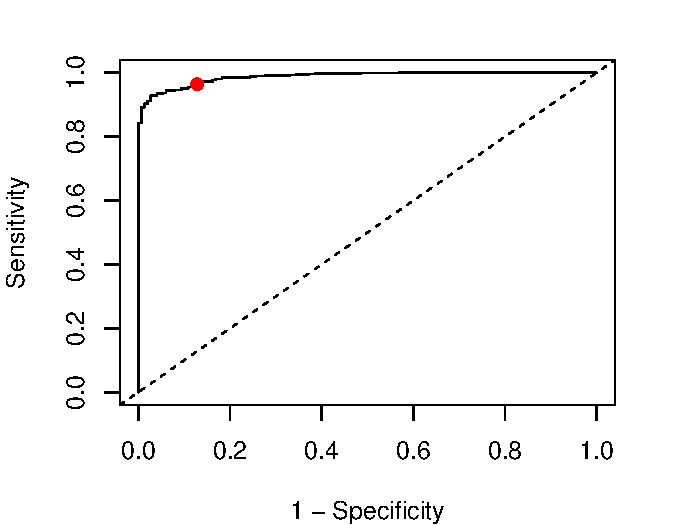
\includegraphics[scale=0.6]{ROC1.pdf}
\end{figure}
\end{frame}

% --------------------------------------------
\begin{frame}{ROC Curve}
\begin{itemize}
\item The point (0,1) in the top-left corner represents perfect classification.  That is, it corresponds to correctly classifying all the response data in the test set.
\vspace{5pt}

\item In general, the closer the ROC curve is to the top-left corner, or (0,1) point, the better the model performs at classification. 
\vspace{5pt}
\item On the other hand, a model that makes random classifications would have an ROC curve that lies close to the diagonal, or 1-1 line. 
\vspace{5pt}
\item For the election data, the ROC curve is close to the top-left corner, and thus the logistic regression model appears to be performing well at classification. 
\end{itemize}
\end{frame}

% --------------------------------------------
\begin{frame}[fragile]{ROC Curve}
I used the \texttt{pROC} package to plot the ROC curve (there are other R packages one could use).  Here's the code:
\small
\begin{verbatim}
> library(pROC)
> roc_obj <- roc(county_votes16_test$trump_win, probs_test)
> plot(1 - roc_obj$specificities, roc_obj$sensitivities, type="l",
       xlab = "1 - Specificity", ylab = "Sensitivity")
# plot red point corresponding to 0.5 threshold:
> points(x = 19/148, y = 758/786, col="red", pch=19) 
> abline(0, 1, lty=2) # 1-1 line
\end{verbatim}
Note that the second argument of \texttt{roc()} are the predicted \textbf{probabilities} on the test set.
\end{frame}

% --------------------------------------------
\begin{frame}[fragile]{AUC}
\begin{itemize}
\item Another popular classification metric is the \textbf{area under the ROC curve (AUC)}.  
\vspace{5pt}
\item The closer the AUC is to 1 the better the model performs at classification.  While a model that performs no better than random guessing would have an AUC close to 0.5.
\vspace{5pt}
\item One reason the AUC is such a popular metric is because it does not depend on a probability threshold.
\vspace{5pt}
\item For the election data, the logistic regression model has an AUC that is close to 1.  We can compute the AUC using the \texttt{pROC} package:
\begin{verbatim}
> auc(roc_obj)
Area under the curve: 0.9876
\end{verbatim}
\end{itemize}
\end{frame}

\end{document}
